\documentclass[master.tex]{subfiles}

\begin{document}

\section*{C. Approach}

\subsection*{Aim 1: Study the effect of emotional value on the extent and
  symmetry of the temporal window of memory linking.}

\begin{figure}[!b]
  \centering 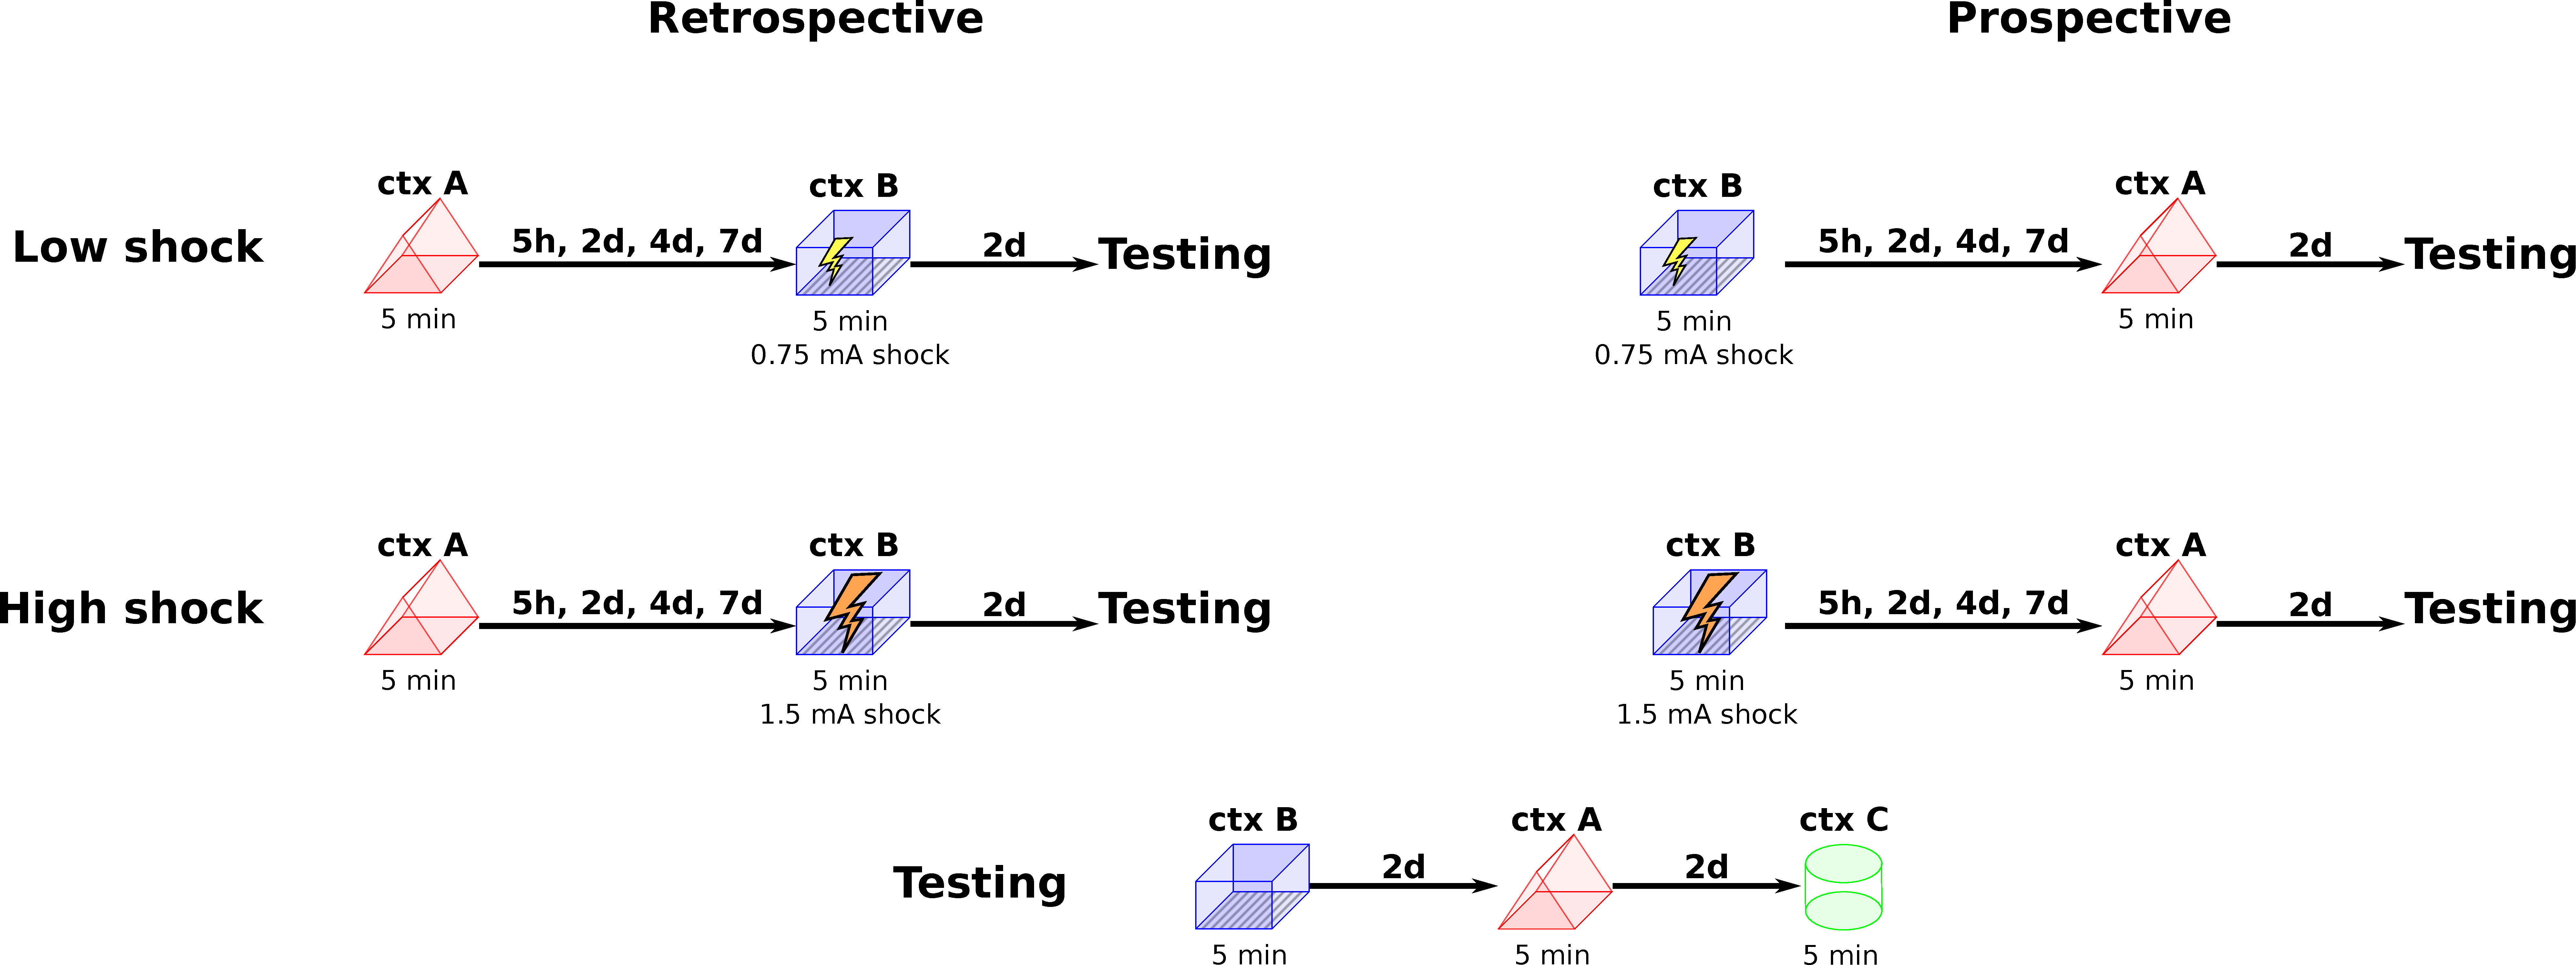
\includegraphics[scale = .135]{Figures/full.pdf}
  \caption{\footnotesize behavior experimental design}
  \label{fig1}
\end{figure}

To test the hypothesis, we will carry out experiments utilizing contextual fear
conditioning. We choose contextual fear conditioning because it is a robust and
well-established test for long-term memory, and moreover a strong memory can be
formed within one learning session.

The experimental design is shown in \autoref{fig1}. Specifically, animals will
be divided into four groups according to two factors: the shock intensity and
the temporal order of the contexts. Two of the four groups receive ``low
shock'', while the other two groups receive ``high shock''; At the same time,
two of the four groups are assigned to ``prospective'' experiments, while the
other two groups are assigned to ``retrospective'' experiments. Thus, overall
the four groups form a 2 by 2 matrix, where groups on the same rows receive same
amplitude of shock, and groups on the same column experience contexts in the
same order. This design allow us to easily compare between groups, and uncover
both the effects and interactions of emotional valence and temporal order.

In all groups, context A, B and C are distinct contexts that differ in lighting
conditions, arena shapes, floor textures and scents. For ``retrospective''
experiments, animals are first put into context A to explore for 5 minutes. Then
after a variable time intervals, the animals are put back into context B for 5
minutes, where they receive a delayed shock at fourth minute with an amplitude
of either 0.75 mA or 1.5 mA, depending on whether the animals are in ``low
shock'' or ``high shock'' group. The variable time intervals are achieved by
further dividing animals into sub-groups according to different time intervals,
and between-group comparison can be carried out. 2 days after these, the testing
sequence is carried out, where the animals are put back to context A, B and C in
that order, with 2d interval in between. Animals' freezing levels are assessed
from behavior video recordings using standard software. For ``prospective''
experiments, the contexts, time intervals, shock intensity assignments and
testing sequence remain identical to those in ``retrospective'' experiments. The
difference is that in ``prospective'' experiments, the animals are first put
into context B, where they receive a delayed shock, and then put into the
neutral context A to explore.

According to preliminary results, we expect to see that in ``low shock'' and
``retrospective'' groups, animals are able to link context A and B together when
they are separated by either 5 hours or 2 days, but not when they are separated
by 4 days or 7 days. Specifically, within ``low shock'' and ``retrospective''
group, we expect to see higher freezing in context A for 5 hours and 2 days
sub-group, but not for 4 days or 7 days sub-group. Similarly, we expect in ``low
shock'' and ``prospective'' groups, the animals are only able to link together
context A and B when they are separated by 5 hours, but not when they are
separated by either 2 days, 4 days or 7 days. Such result would suggest that
retrospective memory linking has longer temporal window than prospective memory
linking. On the other hand, we expect to see in ``high shock'' and
``retrospective'' group, the animals may be able to link context A and B across
either 5 hours, 2 days or 4 days, but not 7 days. Such result would suggest that
more negative emotional value of a memory can extend the memory linking time
window retrospectively.

\subsection*{Aim 2: Study the neuronal correlate of memory linking.}

To study the neural correlate of memory linking, we would carry out miniature
calcium imaging in behaving animals. We choose miniature calcium imaging due to
its capability to record neuronal activities in behaving mice and to track same
field-of-view across long period of time, which is essential for the purpose of
memory linking studies. We will focus on recording in dorsal CA1 region since it
is believed to make a major contribution to contextual memory. The experimental
design is identical to Aim 1 as shown in \autoref{fig1}. Neuronal activities
would be recorded during all experiment sessions to allow collection of rich
dataset.

The raw videos from calcium imaging recording could be processed with an
open-source analysis toolkit CaImAn implementing a constrained non-negative
matrix factorization algorithm. After the process, a spatial matrix representing
the spatial footprint of each putative neurons, as well as a temporal matrix
representing the calcium traces of each putative neurons will be extracted from
the raw data. A custom-written script is used to visually assess the accuracy of
the extraction as well as manually refine the results. After this, neurons from
different recording sessions are cross-registered based on the euclidean
distances between the centroids of their spatial footprint, and a unique master
index can be assigned to each neuron in the whole experiment.

The main comparison is the ensemble overlap between context A and B, B and C, as
well as A and C during retrieval/testing. We expect to see a higher overlap
between context A and B when the two context are linked together and animals
exhibit elevated freezing level in both of them, while the overlap between A and
B are not expected to be significantly higher than those between B and C or A
and C when the two contexts are not linked together.

In addition, a PCA analysis can be carried out to reveal temporal structures of
each ensemble. Specifically, for each recording session, given a matrix
representing the calcium traces of $N$ neurons along $T$ time-steps (usually
frames), a PCA analysis can be applied to extract $R$ principal components,
where each components contain a ``neuron vector'' $\vec{n}$ of length $N$, and a
``temporal vector'' $\vec{t}$ of length $T$. Thus the dimension of the data is
reduced from $N \times T$ to $R \times (N + T)$. The PCA is carried out in a way
so that:
\begin{inparaenum}[a)]
\item the ``neuron vector'' of each principle component represent a group of
  neurons that has a highly correlated firing pattern, and the ``temporal
  vector'' represent that averaged pattern treating the whole group as single
  neuron.
\item a dot product can be computed with each ``neuron vector'' and ``temporal
  vector'', and the sum of $R$ such dot products should closely reproduce the
  original $N \times T$ data.
\item the $R$ components should explain most of the variance in the original
  data, thus the value of $R$ can be determined by thresholding the proportion
  of variance explained.
\end{inparaenum}

Once the principal components of each recording sessions are extracted, we can
calculate a cross-correlation of the ``neuron vector''s between any two session.
We can then compare such correlation matrices between linked context and
unlinked contexts. We expect to see higher correlations between linked contexts,
suggesting that the temporally correlated structures within each ensemble are
more likely to be preserved across linked contexts than across unlinked
contexts.

The presented approach has two caveats that might require further refining:
Firstly, a method to assess the quality of cross-registration is lacking. For
this issue, an algorithm developed by Yaniv lab might be more suitable since it
can also output the confidence of cross-registration. However, as long as the
current approach does not produce systematic bias towards linked contexts, that
is, as long as the field-of-view of recordings remain relatively stable, there
is no reason to expect a significant artifact from presented methods. Secondly,
the application of PCA analysis presume that the neuronal ensembles are
structured such that subsets of cells fire together. It may fail to detect other
temporal structures, such as sequence of firing. For this, other dimension
reduction algorithms might address the issue.
\end{document}
